\documentclass[12pt, twoside, a4paper]{report}
\pagestyle{headings}
\pagestyle{empty}
\usepackage{indentfirst}
\usepackage{graphicx}
\usepackage[english, greek]{babel} % mine
\usepackage[utf8x]{inputenc}  % mine
\usepackage{makeidx}  % mine
\usepackage[nottoc]{tocbibind}  % mine
\usepackage{babelbib}  % mine
\makeindex  % mine

\begin{document}
\selectlanguage{greek} % mine

\title{
\vspace{-6ex}
\begin{center}

\includegraphics[scale=1]{pyrforos.png}  % mine -- no .eps files with pdflatex
\end{center}
\Large{Ε}\large{ΘΝΙΚΟ}
\Large{Μ}\large{ΕΤΣΟΒΙΟ}
\Large{Π}\large{ΟΛΥΤΕΧΝΕΙΟ} \\
\normalsize{Τ}\small{ΜΗΜΑ}
\normalsize{Η}\small{ΛΕΚΤΡΟΛΟΓΩΝ}
\normalsize{Μ}\small{ΗΧΑΝΙΚΩΝ}
\normalsize{Κ}\small{ΑΙ}
\normalsize{Μ}\small{ΗΧΑΝΙΚΩΝ}
\normalsize{Υ}\small{ΠΟΛΟΓΙΣΤΩΝ} \\
\vspace{2ex}
-ΕΙΣΑΓΕΤΕ ΤΟΝ ΤΟΜΕΑ- \\
-ΕΙΣΑΓΕΤΕ ΤΟ ΕΡΓΑΣΤΗΡΙΟ- \\
\vspace{8ex}
\large \textbf{-Εισάγετε τον τίτλο της διπλωματικής εργασίας-} \\
\vspace{10ex}
\large
ΔΙΠΛΩΜΑΤΙΚΗ ΕΡΓΑΣΙΑ \\
\vspace{2ex}
\normalsize
-Εισάγετε το σωστό άρθρο (της/του/των)- \\
\vspace{2ex}
\parbox[c]{0.4\textwidth} { \center\textbf{
-Εισάγετε το όνομα, αρχικό πατρώνυμου και επωνυμο των συγγραφέων- }}
\selectlanguage{english}  % mine -- to make sense
\parbox[c]{0.4\textwidth} { \center\textbf{
	-another author, whose name is here- }}
\selectlanguage{greek}  % mine again
\vspace{10ex}
\flushleft
\begin{tabbing}
	\textbf{Επιβλέπων}: \= -Εισάγετε το όνομα, αρχικό πατρωνύμου
				και επίθετο- \\
			    \> -Εισάγετε τον τίτλο του επιβλέποντα-
\end{tabbing}
}
\date{
\normalsize
Αθήνα, -Εισάγετε το μήνα και το έτος κατάθεσης της εργασίας-}

\maketitle
\newpage
\hspace{10pt}
%\tiny
%(this page is left intentionally blanc)
%\normalsize
% \newpage

\includegraphics{pyrforos.png}  % mine -- no .eps files with pdflatex
\noindent
\parbox[b]{0.6\textwidth} {\textbf{
\noindent
\normalsize{Ε}\small{ΘΝΙΚΟ}  % mine -- this needs modification
\normalsize{Μ}\small{ΕΤΣΟΒΙΟ}
\normalsize{Π}\small{ΟΛΥΤΕΧΝΕΙΟ}} \\
\small
ΤΜΗΜΑ ΗΛΕΚΤΡΟΛΟΓΩΝ ΜΗΧΑΝΙΚΩΝ ΚΑΙ ΜΗΧΑΝΙΚΩΝ ΥΠΟΛΟΓΙΣΤΩΝ \\
-ΕΙΣΑΓΕΤΕ ΤΟΝ ΤΟΜΕΑ- \\
-ΕΙΣΑΓΕΤΕ ΤΟ ΕΡΓΑΣΤΗΡΙΟ-}

\begin{center}
\vspace{8ex}
\large \textbf{-Εισάγετε τον τίτλο της διπλωματικής εργασίας-} \\
\vspace{10ex}
\large
ΔΙΠΛΩΜΑΤΙΚΗ ΕΡΓΑΣΙΑ \\
\vspace{2ex}
\normalsize
-Εισάγετε το σωστό άρθρο (της/του/των)- \\
\vspace{2ex}
\parbox[c]{0.4\textwidth} { \center\textbf{
-Εισάγετε το όνομα, αρχικό πατρώνυμου και επωνυμο των συγγραφέων- }}
\selectlanguage{english}  % mine -- to make sense
\parbox[c]{0.4\textwidth} { \center\textbf{
	-another author, whose name is here- }}
\selectlanguage{greek}  % mine again
\vspace{10ex}
\flushleft
\begin{tabbing}
\textbf{Επιβλέπων}: \= -Εισάγετε το όνομα, αρχικό πατρωνύμου
			και επίθετο- \\
		    \> -Εισάγετε τον τίτλο του επιβλέποντα-
\end{tabbing}
\end{center}

\noindent
Εγκρίθηκε από την τριμελή εξεταστική επιτροπή την -εισάγετε ημερομηνία-.

\begin{center}
\scriptsize
\parbox[b]{0.3\textwidth} {\center
	........................................
	-Εισάγετε ονοματεπώνυμο-
	-Εισάγετε τίτλο-
}
\parbox[b]{0.3\textwidth} {\center
	........................................
	-Εισάγετε ονοματεπώνυμο-
	-Εισάγετε τίτλο-
}
\parbox[b]{0.3\textwidth} {\center
	........................................
	-Εισάγετε ονοματεπώνυμο-
	-Εισάγετε τίτλο-
}
\end{center}
\vspace{10ex}
\normalsize
\noindent
Αθήνα, (εισάγετε το μήνα και το έτος κατάθεσης της εργασίας).
\newpage
\hspace{10pt}

\vspace{30ex}
\noindent
................................... \\
\textbf{(Εισάγετε όνομα, αρχικό πατώνυμου και επίθετο συγγραφέα)} \\
(Εισάγετε τον απονεμηθέντα τίτλο στο συγγραφέα) \\
\vspace{8ex}

\noindent
................................... \\
\textbf{(Εισάγετε όνομα, αρχικό πατώνυμου και επίθετο συγγραφέα)} \\
(Εισάγετε τον απονεμηθέντα τίτλο στο συγγραφέα) \\
\vspace{8ex}

\noindent
................................... \\
\textbf{(Εισάγετε όνομα, αρχικό πατώνυμου και επίθετο συγγραφέα)} \\
(Εισάγετε τον απονεμηθέντα τίτλο στο συγγραφέα) \\
\vspace{26ex}

% mine
\newpage
\tableofcontents
\listoffigures
\listoftables

% here go the \include commands (chapters etc, if you want to do it separately)
% \include{abstract}
% \include{ch0}
% \include{ch1}
\selectlanguage{english}
\def\<#1>{\textit{#1}}

\chapter{FIFO Queues}
\section{Introduction}

FIFO Queues are one of the most widely used data structures. They have been studied thoroughly and are used in many projects. In order to maintain the coherence of the data structure in a multithreaded environment, synchronization between threads is needed. Queues are a structure that, by its nature, allows low levels of concurrency, since all reads and writes are applied on Head and Tail, rendering these locations as hotspots. Therefore, we expect low scalability, as the number of parallel threads increases.

However, in many applications, there is the need of having multiple threads, communicating through a shared queue, that is often needed to serve millions of operations per second. For this reason, concurrent FIFO Queue implementations attract theoretical, as well as practical interest. 

Given the low level parallelization offered by the structure, the problem of high performance, essentially becomes the problem of finding a low cost synchronization scheme, as well as achieving better cache utilization.

\subsection{Global Lock}
In our first implementation we adopted a naive, coarse grained strategy. We introduce a global lock, which every thread is trying to set at the beginning of an enqueue or a dequeue. As expected,  performance is disappointing and the implementation does not scale. The reason is that, only one thread can execute an operation on the structure every given time, while all the other threads spin on the lock. Even after we implemented and used a TTES( Test an TEst and Set) lock that reduces traffic due to the cache coherence protocol, delays were still high.

Another characteristic behavior is that throughput declines dramatically when the number of parallel threads exceeds the number of available cores. In this case, more than one threads share the same core and if a thread holding the lock is scheduled out, no other thread is advancing until that threads regains the cpu and unsets the lock. This is a general problem with locking implementations: If a thread inside the critical section is delayed, the progress of all other threads is halted and performance suffers significantly.

%global benchmark here??

For this reason, in the field of data structures in general and FIFO Queues in particular, great effort has been applied to come up with sustainable, lock free implementations. The first and most well known, successful implementation of a lock-free FIFO Queue is from Michael and Scott \cite{msqueue} and it serves as a base line for all further efforts.

\section{Michael Scott Queue}
\subsection{Description}

The data structure is implemented as a simply linked list, with a pointer Head referencing the start of the list, where dequeues are applied and a pointer Tail at the end where we can add new nodes. The node pointed by Head is considered a dummy node  and is used to ensure that the list is never left empty.

In its core, the algorithm uses atomic operations ( in particular Compare And Swap operations) to atomically modify the appropriate pointers. Every time, we run checks to make sure that we have a consistent view of the pointers we are trying to modify.

As depicted below, an enqueue requires 2 atomic operations: one to link the last node with the new node we are trying to insert and one to swap the Tail pointer to the new node.

% εικόνα 1 από το optimistic paper
\begin{figure}
 \centering
  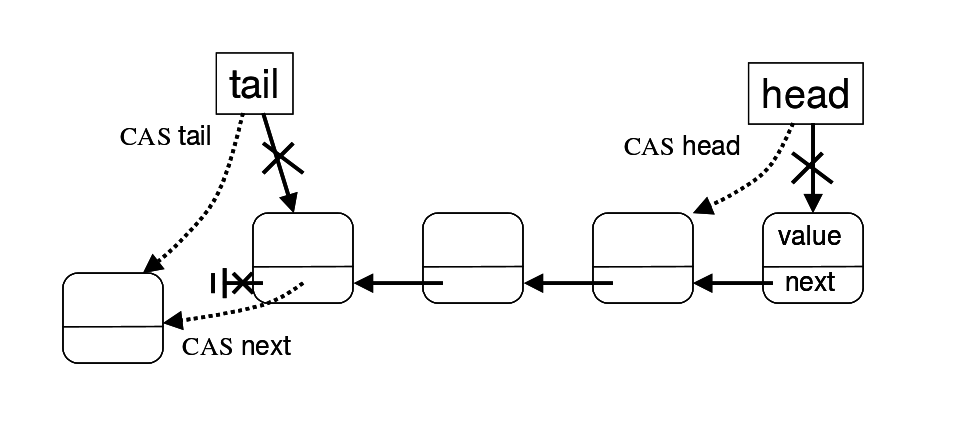
\includegraphics[scale=0.4]{msqueue_struct.png}
\caption{ The basic layout of the link list used in Michael Scott implementation}
\end{figure}

On the other hand, we need only one C-A-S on the value of Head to perform a dequeue.

\subsection{Challenges}
At any given time during the execution of a thread, the values of Head and Tail can change unexpectedly, causing the atomic operations to fail and the execution to start over from the top: read the new value of Head/Tail and try to change it atomically. Moreover, in order for an enqueue to finish, both two required C-A-Ss need to succeed. This in turn makes it possible for the new node to be added to the list, without updating the value of Tail accordingly, i.e. Tail doesn't point to the last node. For  this reason, during enqueue or dequeue, it is necessary to check for this inconsistency and correct it.

One of the problems that occurs during the implementation of this algorithm in particular and of algorithms that use C-A-S in general, is the so called ABA problem. In summary, the problem is described by the following scenario: A process observes that a memory location is in a state A and then is halted for a while. In the meantime, another process alters the state of the memory location to B, then back to A again. The initial process will find that the state of the memory location is A and a CAS will succeed, without knowing that the state has changed in the meantime. This problem is related to the lack of a garbage collector that would ensure that we could not release a memory segment that is still being referenced by a thread.

In order to solve the problem, we chose to use modification counters, which we increase on every successful C-A-S and we incorporate them along with every pointer on the data structure. Atomic operations are now performed, not on the pointer but on the pair <pointer, modification counter> which is now treated as a single variable. Thus, we now have to treat pointers in a non traditional way, extracting them from the variable using bit shifting. Alternatively,  there have been put forward many ways to solve the ABA problem, for example with the use of reference counters, that doesn't require merging counters and pointers.

\subsection{results}
The result is a lock-free implementation,  that does not require central locking of the data structure and allows all threads to advance. Performance is not affected by random delays that a thread can have. It thus improved performance compared to the global lock implementation, especially when the number of concurrent threads exceeds the number of available cores.

% isws grafikh gia msqueue

%lock-freeness/orthothta?


\section{Optimistic Queue}

\subsection{introduction}
One of the drawbacks of lock-free approaches is that, each time an atomic operation fails, the execution start back from the top. Moreover, failed atomic operations are costly, due to the synchronization barrier they introduce. Especially in Michael Scott Queue, since both two atomic operations need to be successful in order to complete an enqueue, it is quite common for a thread to repeat execution again and again until it is done correctly. For this reason, we would like to reduce the number of synchronization points ,e.g. the number of atomic operations.

A solution to this problem is introduced by the next algorithm we implemented, by Ladan-Mozes and Shavit \cite{optimistic}. This implementation follows an optimistic approach ( which is why we will refer to this implementation as optimistic queue), in a sense that it runs quickly on the optimistic case where there is no conflict and leaves the costly operations for the case where an inconsistency is spotted. In particular, one of the two C-A-S operations, during enqueue, is replaced with a simple local store, making sure that we correct the data structure in case it is inconsistent.

\subsection{implementation}
Practically, the link list becomes a doubly linked list, with the "next" directions being from Tail to Head. In this way, we only need a single C-A-S to Tail to make it point to the new node, in order to successfully complete an enqueue. However, in order to have access to node from head when we dequeue, we need pointers in the reverse order, as seen below.

%figure 2 apo optimistic paper
\begin{figure}
 \centering
  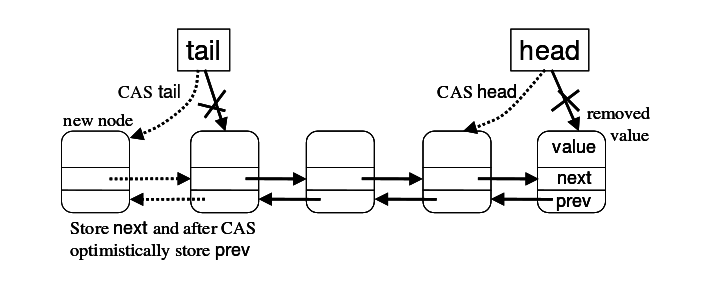
\includegraphics[scale=0.6]{optimistic_struct.png}
 \caption{ The basic layout of the doubly linked list used in the Optimistic Queue}
\end{figure}

Pointers in both directions are updated with simple local stores , without synchronization, which makes inconsistencies possible, in the "prev" direction. For this reason, as soon as an inconsistency is spotted, function FixList is called to traverse the list and fix all the pointers. However, the reason for inconsistencies in the "prev" direction are the long delays a single thread might take and not contention. Therefore, we expect the number of calls to FixList to remain low, even when the number of parallel threads increases.

Inserting a new node in the list includes 3 steps:
1) Set the next pointer of the new node we are trying to insert
2) Compare And Swap on Tail, to make it point to the new node
3) Change the prev pointer of the next node.

\subsection{ABA and consistency}

In order to avoid the ABA problem and spot inconsistencies, this implementation also uses modification counters, that are merged along with the pointers and are incremented in every successful C-A-S

Any thread might take arbitrary time  between steps 2 and 3 and during this time more nodes might be inserted in the queue. Note however that, every time a node is successfully inserted in the queue(after successful C-A-S), the modification counter to be inserted next is incremented by one. Thus, pointers of consecutive nodes in the queue, will have consecutive modification counters. In this way, during a dequeue, if a prev pointer does not have the expected modification counter, FixList is called and the pointers are repaired.

Note that there must be special care taken to ensure that there is always one dummy node in the list and Tail never goes past that node.

\subsection{Failed C-A-S operations}

The next diagram compares the number of C-A-S operations( both successful and failed) needed to execute 1 million pairs of enqueue/dequeue, across these two lock-free implementations. We can see that the optimistic approach, as promised, requires less C-A-Ss and has, in total less costly, failed C-A-Ss as the level of concurrency increases.

%διαγραμμα για failed CAS
\begin{figure}
 \centering
  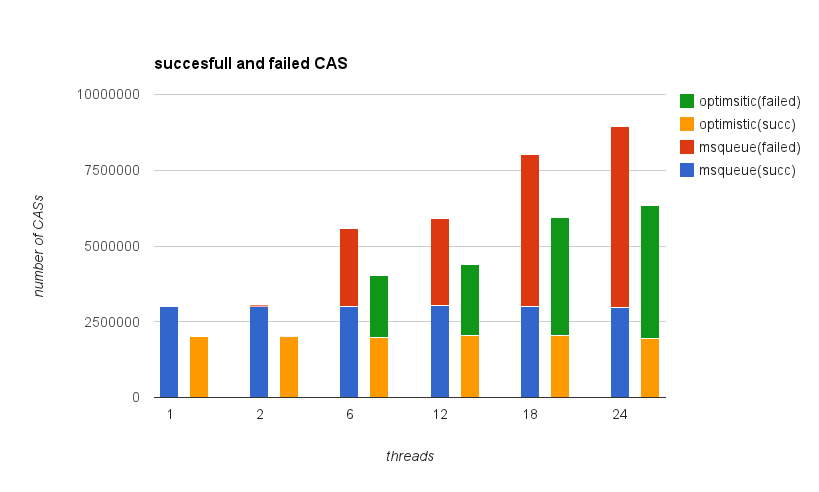
\includegraphics[scale=0.5]{failed_cas.png}
\caption{Total successful and failed C-A-Ss for the two lock-free implementations}
\end{figure}

\section{Flat Combining}
\subsection{Introduction}

The two proceeding implementations follow a fine thread approach, where every thread has access to the data structure and they are trying to achieve performance through high parallelization. As more treads are free to operate on the data structure, performance is expected to be better that locking approaches that block the progress of some threads. We next present the principles of flat combining, a programming approach by Hendler, Incxe and Shavit \cite{flat_combining} that goes against the above mentioned statements.

In particular, the authors claim that the point at which the cost of synchronization between threads exceeds the benefit from high parallelization, is at a lower lever of concurrency than expected. Flat combining is based on a synchronization scheme where each thread locks  the data structure in an extremely low-cost way, gathers information on the operations trying to be executed on the queue by the other threads and then does the operations in their place. The result is an implementation with low synchronization cost and better cache performance, overcoming the drawbacks of blocking and low parallelization.

\subsection{Implementation}

Flat combining is a layer of abstraction that can be used over a sequential structure and its basic functions is the following:
1) Every thread publishes the operations it is trying to perform on the structure, along with any parameters, on its corresponding public record. These records can be in an array, for fast read/write or in linked list with dynamic size, proportional to the number of active threads.
2) Every thread checks the state of the locks and if it finds it unlocked, it tries only once to atomically set the lock. If the lock was locked already, the thread spins in its public record, waiting for a response.
3) If it takes the lock, this thread is considered the new combiner. It then traverses the public records and executes the request on the data structure, one by one, writing back the results. Finally the thread releases the lock.

% isws kana sxhmataki  gia th domh  san auto sto paper

\subsection{Implementation characteristics and Benefits}
From the way flat combining works, certain advantages can be concluded:
1)Since only the combiner has access to the structure, operations can be optimized with the best sequential algorithm, without minding synchronization and concurrency. This even allows us to implement concurrent structures, such as pairing heaps, that are otherwise difficult to implement using fine grain synchronization, by applying flat combining over already existent sequential data structures.
2) in some cases, the combiner can use some smart way to group the request and make the access to the structure faster and more efficient. For example, in concurrent stacks, a combiner can perform elimination between a concurrent enqueue and a concurrent dequeue. In our queue implementation, we used fat nodes to group data, as we explain later on.
3) The combining way of accessing the structure can lead to better cache utilization.
4) Using a global lock to isolate the structure makes programming, as well as debugging, much easier.

It is also important to note that flat combining, as a layer of abstraction that ensures synchronization, can bee used as it is over different data structured. Of course, not all data structures are benefited by flat combining. For example, if the cost of a single operation in a search tree is \textgreek{Θ} (logn), using flat combining, the cost of k operations is in general \textgreek{Θ} (klogn), while we could  use parallel threads that execute operations independently on different parts of the tree in \textgreek{Θ} (longn) total time.

FIFO Queues in particular, seem to benefit by flat combining, given that they already allow low levels of concurrency ( only two access points). In our implementation, we organized public records in an array and used fat nodes, where every node can hold up to 16 values. Therefore, we only need to add one node in the queue and swap the Tail pointer only once, for every 16 values inserted. We also used two independent instances of flat combining, one for enqueues and one for dequeues, in order to exploit the maximum concurrency allowed.

\subsection{First results}
 %grafikes gia fc se sxesh me ta alla
 
\subsection{Optimizations}
%1 dedicated combiner
From the analysis of the algorithm we can deduct that every thread can, in theory, access the queue and alter its state. That means that the nodes of the queue can be in the cache memory of any thread, which in turn leads to increased cache misses and long delays.

For this reason, we alter the existing implementation, so that only a given thread for each operation(enqueue/dequeue) can become a combiner. Essentially, all threads are being server by only two specific threads. These two threads have less cache misses when they access the structure.

The result is a constant improvement in performance, that corresponds  to less cache misses and better locality. Specifically on dunnington, this improvement is even more apparent.

%2 hybird
We next  studied the behavior of these algorithms in NUMA architectures. From the general performance of these algorithms, it is obvious that when threads are no longer contained in one NUMA node, performance suffers significantly, due to the fact that threads no longer share the same L2 cache. Moreover, atomic operations and specifically Compare-And-Swap), are much more costly when they need to synchronize threads that belong to different NUMA nodes.

The previously implemented flat combining algorithm is not NUMA-aware and cannot deal with the problems mentioned above. For this reason, we designed and implemented a hybrid implementation that combines previous algorithms, taking architecture into account, in order to achieve better performance.

The implementation that was eventually chosen  consists of two stages. In the first stage, we use flat combining in every NUMA node. Threads of the same node are synchronized to come up with a combiner. In the second stage, combiners from each node are further synchronized to access the queue. In the second stage we tried several synchronization schemes ( Michael-Scott queue, a second level of flat combining). Eventually, the best performance for the given architecture was achieved by a simple TTAS global lock.

The result was a further improvement of the performance,



\selectlanguage{english}
\def\<#1>{\textit{#1}}

\chapter{Hash Tables}
\section{Introduction}

Hash Tables are a fundamental data structure that provides fast store and lookup operations, and it is used in various programming applications. The ability ,for example ,to create sets and quickly perform searches on them, depends on the efficiency of the underlying Hash Table. For this reason, many algorithms and approaches, both sequential and concurrent have been put forward, each with its own distinctive strengths and weaknesses. 

The purpose of a Hash Table is to efficiently associate a given value with a key and use that key to rapidly store or search that value among other values. It usually consists of an array or list of buckets, which can hold one or more values, as well as a hash function that maps a value on the table.

Ideally,  every different values will hash to different buckets, making it easy to insert and search them, However, it is improbable that there will be no collisions, in fact for a large number of operations we expect collisions to be quite common. For the purpose of avoiding collisions, one must consider the size of the hash table (more buckets  means more ways to distribute the keys) and the hash function ( a hash function that will evenly distribute keys among the available buckets will reduce collisions). Even so, collisions are unavoidable, and the way they are handled is one the most important factor among the various implementations.

\subsection{Collision Resolution}

Hash tables can be divided into two main categories: Closed Addressing and Open Addressing.

%add some bullets here

Closed addressing hash tables allow more than one values to be stored on the same bucket. This is usually implemented by attaching a linked list at the start bucket , and each new value is added on the list. The length of the list  must be kept bellow a constant number (called load factor) , to keep operations on the list fast. This way the average lookup / insertion time is dependent only on load factor. It is common to keep the list ordered , which reduces the average lookup time in half. This is an easy to implement data structure and it has been proven to perform well in practice.

Open addressing hash tables allow no more than a single value per bucket. When a collision is detected, the buckets are traversed in order to find an empty bucket to store the new value, even though it’s hash value does not correspond to that bucket. The sequence according to which the buckets are traversed is typically:

1) Linear probing, where an empty bucket is searched within a given number of steps from the mapping bucket
2) Quadratic probing, where the buckets is searched at increasingly bigger intervals, according to successive values of a quadratic polynomial. 
3) Double hashing, where interval is the outcome of a new hash function.

% kapoia sxhmata edw

 Some other important techniques used in resolving conflicts in open addressing hash tables is cuckoo hashing and hopscotch. Cuckoo hashing, as explained later in detail, employs a second , or more hash functions. The value is first hashed using the first hash function  and if it corresponds to an non-empty bucket the second hash function is used. If both buckets are empty, then one of the two previously hashed values is evicted and then hashed again using the other hash function, possibly triggering a series of evictions until all values are hashed.

%sxhma gia cuckoo hashing 

Hopscotch hashing combines linear probing and cuckoo hashing. First , buckets are traversed until an empty bucket is found. If that bucket is in the neighborhood of the initially mapped bucket, the value is placed there, just as in linear probing. If the empty bucket is outside the neighborhood, values are moved in a sequence of hops, effectively moving the empty slot closer and closer to the neighborhood of the initial bucket. An example is shown at figure \ref{fig:hopscotch_hashing}.

%sxma gia hopscotch hasing
\begin{figure}
 \centering
  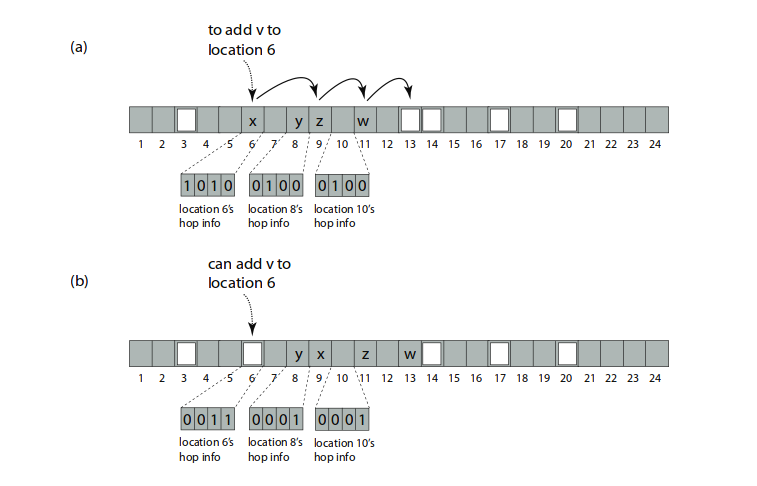
\includegraphics[scale=0.5]{hopscotch_hashing.png}
\caption{Example of an insertion in hopscotch hashing. Here we try to insert value 6 and the first empty bucket is found at index 13, outside the neighbourhood of bucket 6. We then find out that w an index 11 can be displaced to the empty bucket and we place it there. Now the empty bucket is at index 11 wich is still far from 6. Subsequently, by switching places with buckets 9 and 6, the empty bucket is finally at index 6 and the new value can be inserted }
\label{fig:hopscotch_hashing}
\end{figure}


\subsection{Resizing}

Resizing is important to maintain constant average insertion and lookup time. In closed addressing algorithms, buckets may become too full, making their traversal slow, while in open addressing algorithms, the table may become too full to easily  find empty buckets . In either case, the size of the table needs to be expanded and all the values from the old, small hash table must be transferred to the new bigger one. This can be done by rehashing every value of the old table to the new one (possibly causing a high delay which may not be acceptable in a real time application) or  incrementally , by moving every new inserted value to the new table , along with a few elements from the old table each time, until the old table is empty.

\subsection{Concurrent hash tables}

In a multiprocessor environment it is quite common for multiple threads to require concurrent access to the same hash table. Access on disjoin locations on the hash tables, suggests hash tables are may allow a much higher level of concurrency, compared to FIFO queues as studied above. However, keeping the data structure fast and consistent despite contention, introduces many challenges and many diverse concurrent algorithms have been proposed to face them.
   
% edw tha moune oi alles ylopoihseis

\section{ Locking Approaches}

We start by implementing the hash table as a table of nodes, with each node being the head of a simple linked list that we keep ordered. We protect the table with a simple spinlock. Each thread needs to acquire the spinlock before performing any operation ( insert, lookup or delete). 

In order to ensure that every operation takes constant time, we need to keep the average number of items in every link list bellow a minimum. This is done by resizing the table , according to a certain policy. The resizing mechanism may trigger when the number of buckets that have grown beyond a certain threshold is large, or when the total ratio of inserted elements to the number of buckets exceeds a threshold. To perform the resize operation, a thread acquires the lock, checks if another thread has already resized the table and if not, proceeded to allocate a new table twice as big as the old one and then rehash every value from the old table into the new one.

The global lock mechanism is simple to implement but it introduces a sequential bottleneck and performance is low, as shown in figure \ref{hashes_global_perf}. All threads spin on the same lock, even they are trying to access disjoint locations on the table . Moreover , since the critical section inside the lock is very small, the overhead of acquiring and releasing the lock becomes a large proportion of runtime.

\begin{figure}
 \centering
  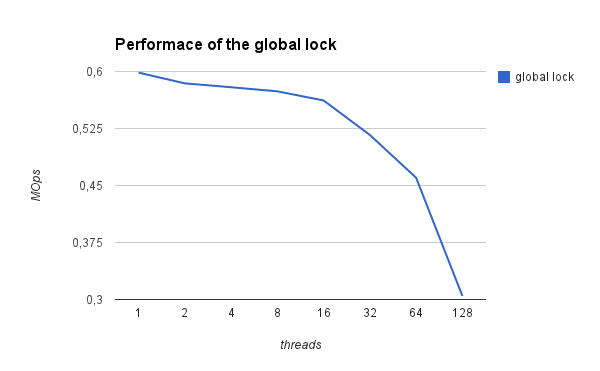
\includegraphics[scale=0.7]{hashes_global_perf.png}
\caption{The performance of the naive global lock approach}
\label{hashes_global_perf}
\end{figure}

We then try to permit more concurrency by used a fixed number of locks , instead of a single one. We introduce an array of spinlocks with length L, with each lock protecting a number of buckets. We determine which lock is responsible for each bucket by simply mapping the index of the bucket on the array of locks. As the table grows, the number of locks remains the same ,so each lock is responsible for more buckets, as shown in figure \ref{striped_hash_set}.

%sxhma apo to vivlio tou shavit
\begin{figure}
 \centering
  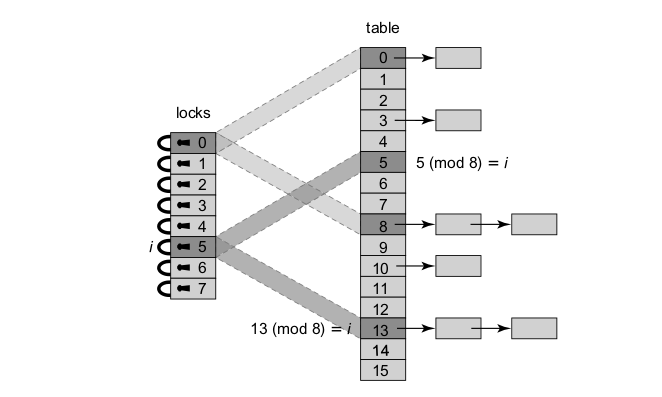
\includegraphics[scale=0.5]{striped_hash_set.png}
\caption{A representation of the striped hash set}
\label{striped_hash_set}
\end{figure}


Having more than one locks means more than one threads can proceed  successfully and this results to less contention, more concurrency and improved performance. Increasing the number of locks , closer and closer to the number of buckets, seems to improve throughput and refuce latecny , as depicted in figures \ref{hashes_striped_through} and \ref{hashes_striped_latency}. However, if we want to keep the number of locks equal to the number of buckets, as the table increases in size, we need to be able to resize the lock array as well, which is not straight forward.

\begin{figure}
 \centering
  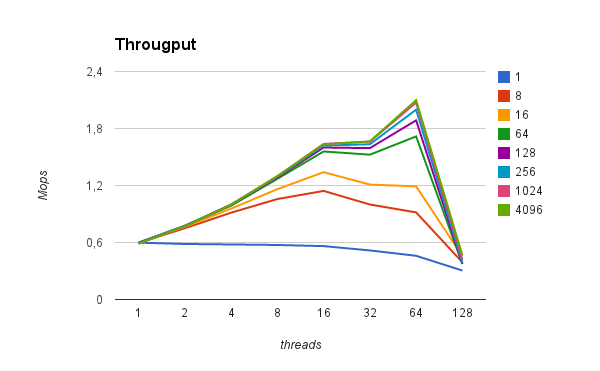
\includegraphics[scale=0.7]{hashes_striped_through.png}
\caption{Throughput for various numbers of locks}
\label{hashes_striped_through}
\end{figure}

\begin{figure}
 \centering
  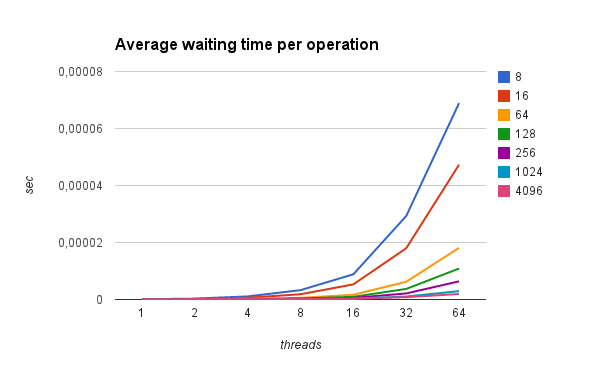
\includegraphics[scale=0.7]{hashes_striped_latency.png}
\caption{Latency for various numbers of locks}
\label{hashes_striped_latency}
\end{figure}
For this reason we then try to implement a refinable locking scheme, where locks can be dynamically increased to match the number of buckets. Here, we require mutual exclusion between resizing and updating, so we introduce a marked field owner, containing the id of the thread that is currently resizing. When a thread is trying to resize, it first atomically sets the mark bit and writes its id in the owner field. It then waits until no more updates are being performed(e.g. all the locks are unlocked). That way, all other threads that are trying to update, will find the marked bit of the owner value set and will not proceed to take any lock. The thread is now free to resize the table and the lock array, rehash every value into the new table and unset the marked bit. In this implementation, we also allow lookups to first search the value without taking a lock. This allows to sometimes successfully perform lookups, even during resizing. If the value is found, lookup returns that value. If not, it might be possible that the value was inserted but the thread could not access it yet, so the thread tries searching again, this time holding the lock. 

The outline of the function used by every thread to acquire a lock is shown here, where we can see how the when the mark bit of the owner field is set, no one can acquire any locks.

\begin{lstlisting}

void acquire(HashTable_t T , int x){
	
	me =  current thread index
	while (1){
		do{
			<who, mark> = owner
		}while (mark && who != me)
		
		Locks[] oldLocks = locks
		lock the apropriate lock on oldLocks array
		<who, mark> = owner
		if ((!mark || (who == me)) && locks = oldLocks)
			return
		else 
			unlock the lock from oldLocks array 
	}
}

\end{lstlisting}

The result is an increase in performance, because we exploit the finer grained syncronization. However, this imporovement comes with the cost of slower resizing. Increasing the number of locks means that we need more time to allocate the extra locks and more time to wait until all locks are free. The extra amount of time introduced is shown in figure \ref{hashes_refinable_resize}.
 
\begin{figure}
 \centering
  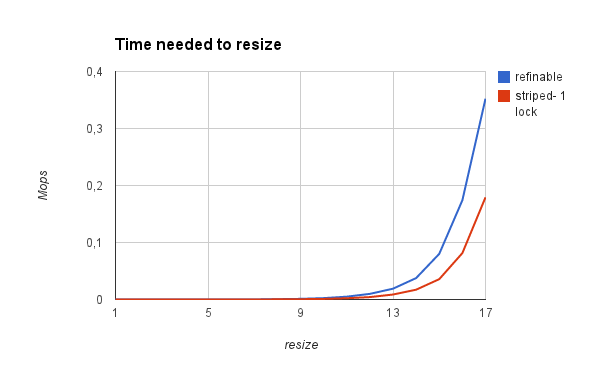
\includegraphics[scale=0.7]{hashes_refinable_resize.png}
\caption{The amount of time needed for every resize}
\label{hashes_refinable_resize}
\end{figure}

\section { Split Ordered List}

All the above mentioned algorithms use locks to enforce synchronization and therefore inherit all the disadvantages of blocking algorithms such as low performance when the number of threads exceeds the number of available cores. Moreover, these algorithms perform resizing in a "stop -the - world" manner, meaning that a single thread resizes the table and during that time no other thread can proceed. We now focus on a lock free algorithm  by  Shalev and Shavit  \cite{split_ordered} ,that uses atomic operations for synchronization and the hash table can grow incrementally without having to rehash any value or introduce a thread barrier.

The algorithm is based on a lock-free linked list , implemented by Michael \cite{lock_free_list} to store the values. The buckets, kept in a single array, are now references to specific nodes in the list, representing the start of the particular bucket, effectively working as short-cuts into the list. As the list grows, we introduce new buckets that split the older ones in half, keeping their size bellow a maximum value. In order to do this however, the list must be kept ordered according to a recursive split order, as described next.

Split ordering is in fact the reverse bit representation of values, kept in ascending order. The goal here is to split each bucket by inserting a new one, without having to rearrange anything else. Figure \ref{split_ordered_1} explains how split ordering achieves just that.

% figure apo th diafania kai exhghsh
\begin{figure}
 \centering
  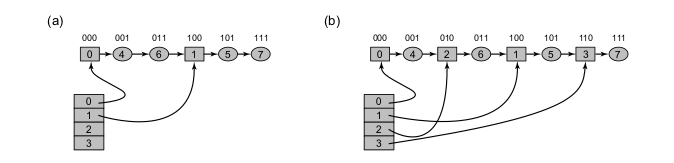
\includegraphics[scale=0.5]{split_ordered_1.png}
\caption{This figure explains how split ordeding manages to effectively split a bucket in half.In part a , the list consists of two buckets. Above each node is it's split-ordered key, which is the reversed bit representation of each value. Square nodes are sentinel nodes, depicting the start of each bucket. When the table capacity grows from 2 to 4 in  part b, two new buckets are inserted, spliting the older one in half}
\label{split_ordered_1}
\end{figure}

There are some extra things to note here that illustrate why this specific type of ordering is the ideal for our need. Imagine a thread trying to search for the value 6 in the hash table depicted in part a. The capacity ( the number of buckets is 2) so and values 6 hashes to bucket zero. The thread starts traversing the list and while being at node value 4, a delay occurs. During that delay, capacity is double and a new bucket (bucket 2) is inserted between values 4 and 6, splitting bucket zero in half. As seen above, 2 is prior to 6 according to split ordering, and that mean that traversal well go past 2 and keep looking until it successfully finds the value 6. This depicts a key idea of the algorithm: when the table's capacity is doubled from 2\textsuperscript{i} to 2\textsuperscript{i+1}, a buckets b is split in half and those elements with values k for witch k mod 2\textsuperscript{i+1} =b  remain in bucket b while the others migrate to bucket b + 2\textsuperscript{i}. The algorithm ensures that these two bucket are positioned one after an other, so that in order to split the bucket we don’t really have to move any node around, but instead we only need to let the new bucket start after the first group of items and before the second.

To avoid the case where a node referenced by a bucket is deleted, we use sentinel nodes, inserted at the lists locations pointed to by every bucket. We use the Least Significant Bit of the reversed bit representation to differentiate between normal node and sentinel node and we don not de-allocate these sentinels node during deletion operation, in order to avoid corner cases.

In order to keep track of the load factor, we update a shared variable on every insert/delete operation that depicts the number of values currently stored in the table. If the ratio of inserted values to number of bucket exceeds a certain limit, we double the capacity, thus introducing new available buckets. Note that, in order to avoid complexity, we allocate a large array of buckets in advance. By introducing an extra level of indirection, namely an array of array of buckets, we are able to adaptable increase the maximum number of available buckets if needed.

Figure \ref{split_ordered_2} is an example of how adding a new value in the hash table increases capacity and introduces new buckets.

% figure gia insert apo diafanies kai exhghsh 
\begin{figure}
 \centering
  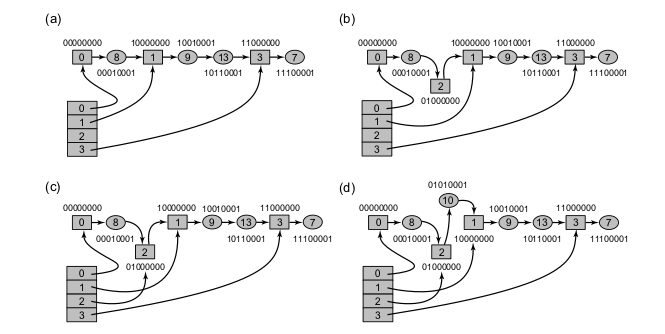
\includegraphics[scale=0.5]{split_ordered_2.png}
\caption{Example of an insertion in the split ordered list. At part a , the bucket 2 is uninitialized. Inserting value 10, initializes the bucket, inserting a sentinel node in the list, before the actuall insertion of 10 at part d}
\label{split_ordered_2}
\end{figure}

Note that unused buckets are uninitialized. The sentinel nodes for each bucket are only inserted when it is actually needed, that is when this buckets holds at least one value. When initializing a bucket, we might also need to recursively initialize other buckets that come before it as shown in figure \ref{split_ordered_3}

% figure gia initialization apo diafanies
\begin{figure}
 \centering
  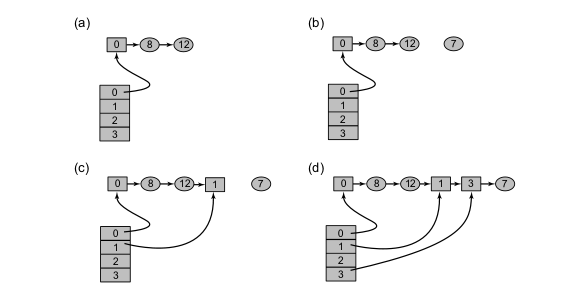
\includegraphics[scale=0.5]{split_ordered_3.png}
\caption{Example of recursive initialization of buckets, before insertion of value 7}
\label{split_ordered_3}
\end{figure}

The insert operations looks very simple, simply initializing the bucket if needed and then insert the split-ordered key in the list starting from the node referenced by the apropriate bucket. Finaly, we check if the capacity need to be doubled. The same outline is followed by the lookup operation.

\begin{lstlisting}

int insert(HashTable_t T, int key){
	node =  allocate new node
	node->key = split_ordered_representation(key)
	bucket = key \% size
	if T[bucket] == uninitialized
		initialize(bucket)
	if (! list_insert(&T[bucket], node)){
		delete node
		return 0
	}
	csize = size
	if (fetch_and_add(&count ,1) / cize > MAX_LOAD)
		CAS(&size,csize, 2 * csize)
	return 1
}

int find(HashTable_t T, int key){
	bucket = key \% size
	if T[bucket] == uninitialized
		initialize(bucket)
	return list_find(&T[bucket], split_ordered_representation(key))
}

\end{lstlisting}

At its lower level, this implementation utilizes a lock free list. Each thread hash a set of three private variables curr, prev and next, each consisting of a pointer to a node, along with a mark bit. These pointers traverse the list to find the appropriate locations for an insertion or deletion and then the thread attempts to atomically modify the list, using Compare And Swap operations

The result, shown in figure \ref{hashes_split_ordered_perf} is a lock free hash table that allows high concurrency, fast operations on the list and most importantly , does not require resizing and rehashing the entire hash table.

\begin{figure}
 \centering
  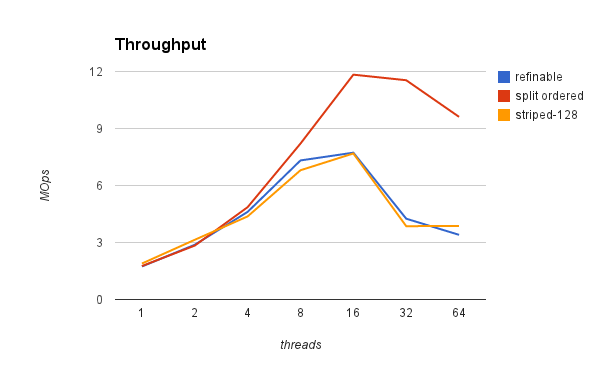
\includegraphics[scale=0.7]{hashes_split_ordered_perf.png}
\caption{Performance of the split ordered algorithm}
\label{hashes_split_ordered_perf}
\end{figure}

\section{Cuckoo Hashing}
\subsection{Sequential version}

We now turn our attention to an open-addressing hash table, called cuckoo hashing. Open-addressing algorithms allow for only one value to be stored at each bucket. In its sequential version, cuckoo hashing uses two arrays of buckets and two hash functions, although it is possible to use only a single array. 

Lookup operations are quite simple. The value is hashed using the first hash function and the corresponding bucket on the first array is checked. If the value is not found, the second hash function is used and the second array is  checked.  If the value its not there either, the lookup operation returns that the value does not exist on the hash table.

The basic idea behind cuckoo hashing is better shown during the insertion operation. We first hash the value using the first hash function and insert it on the appropriate bucket. If that bucket was initially empty, the process is over. If not, the previous value stored in that bucket is evicted, and we then insert it  on the other hash table, using the other hash function, possibly evicting another value in the process and so on, until an empty bucket is found.

% eikona gia cuckoo hashing insertion.. apo pou?
\begin{figure}
 \centering
  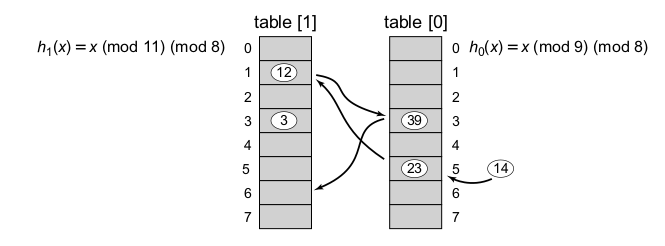
\includegraphics[scale=0.5]{cuckoo_hashing.png}
\caption{Insertion in cuckoo hashing. Trying to insert value 14, we find both apropriate bucket taken by values 3 and 23. Thus, a sequence of displacements is triggered, ending when value 39 is inserted to the previously empty bucket at Table[1][6] }
\end{figure}

The chain of evictions and insertions can grow too long if either the table is too full and no empty buckets can be found easily, or the sequence of displacements form a circle, looping over the same buckets. For this reason, we set an upper limit on the number of evictions triggered by a single insertion. If that limit is exceeded, the table needs to be resized.

There are many variations of the sequential cuckoo hashing algorithms some using more than two different hash function. In general, sequential cuckoo hashing has been proven to work well in practice for a small  to medium load factor.

\subsection{Concurrent version}

In order to implement a concurrent cuckoo hash table, a few changes were maid to the original sequential version. Instead of single element buckets, we use probe sets , whose size is not allowed to grow beyond a certain upper limit. Every set also has a threshold, which is the number of items that can be normally stored inside a bucket. The number of elements stored in a bucket at a given time may exceed the threshold, but the extra elements are marked for eviction and reallocation using the other hash function.

The main principle of the algorithm remains the same. During insertion, the value is added in the set and if the size of the set hash exceeded the threshold, we try to reallocate items using the other hash function and into the other hash table.  In our implementation, we choose to evict the first item on each set, although several other strategies can be chosen instead.

In order to ensure synchronization, we choose to associate every set with its own lock. During any operation (insert, lookup or delete) on a value x, we lock the sets with index h1(x) on table 1 and h2(x) on table 2 accordingly, always in this order, to avoid deadlocks. During resizing, a thread take all the locks on table 1 in ascending order, allocates two new tables, rehashes everything from the old tables to the new ones and releases the locks in the same order. Note that it is possible to implement a striped approach, as discussed in previous implementations, whereas there is a lock-free implementation of cuckoo hashing in the literature \cite{lock_free_cuckoo}.

The basic outline of the insert function is shown bellow.

\begin{lstlisting}

int insert(HashSet * table, int x){
	acquire the locks on both buckets that x maps to
	h0 = hash0(x)
	h1 = hash1(x)
	i=h=-1
	mustResize = false
	search(x) if found return false
	set0 = table[0][h0]
	set1 = table[1][h1]
	if set0.size < THRESHOLD {
		add(set0, x)
		return true
	}
	else if set1.size < THRESHOLD {
		add(set1, x)
		return true
	}
	else if set0.size < PROBE_SIZE {
		add(set0, x)
		i=0 
		h=h0
	}
	else if set1.size < PROBE_SIZE {
		add(set1, x)
		i=1
		h=h1
	}
	else{
		mustResize = true
	}
	if mustResize{
		resize()	
		insert(T,x)
	else if (! realocate(i,h)){
		resize()
	}
	return true
}
		

\end{lstlisting}

%The result is a concurrent open-addressing algorithm that perform extremely well when the load factor is small enough, especially on workloads that consist mainly of lookups.

In the cuckoo algorithm, search is faster because only two buckets with limited number of items must be checked. However, cuckoo hashing usually requires more than half of the table to be empty in order to perform properly. Moreover, some insertions may cause a realoction chain to loop, forcing the table to resize early, meaning that we cannot easily keep the table from expanding without altering the hash functions. As a result we have bigger tables that are resized more often and during resize, memory allocation is undertaken by a single thread while all the others wait doing nothing.

\begin{figure}
 \centering
  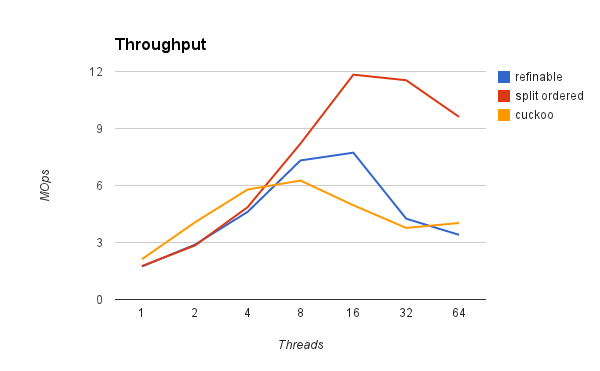
\includegraphics[scale=0.5]{hashes_cuckoo_perf.png}
\caption{Performance of the cuckoo hashing algorithm}
\label{hashes_cuckoo_perf}
\end{figure}

\section{Non Blocking  open addressing}

Last of all, we implemented another open addressing algorithm , introduced by Purchell and Haris \cite{non_blocking_open_addressing} that, unlike cuckoo hashing,  achieves non blocking access by using simple atomic operations.

This algorithm resolves conflicts by using quadratic probing, along the subsequent values of <to polyonymo >.In this implementation, every bucket is accompanied by a probe bound, a value depicting the number of collision on the probe sequence. For example, when searching for a value on a bucket with a probe bound of 4 , we need to take up to 4 steps in the quadratic sequence to search for that value. Keeping a consistent view state of the probe bound can be challenging when multiple threads are inserting or deleting on the chain of collisions, as seen in figure \ref{non_blocking_1}.

% figure2 apo paper
\begin{figure}
 \centering
  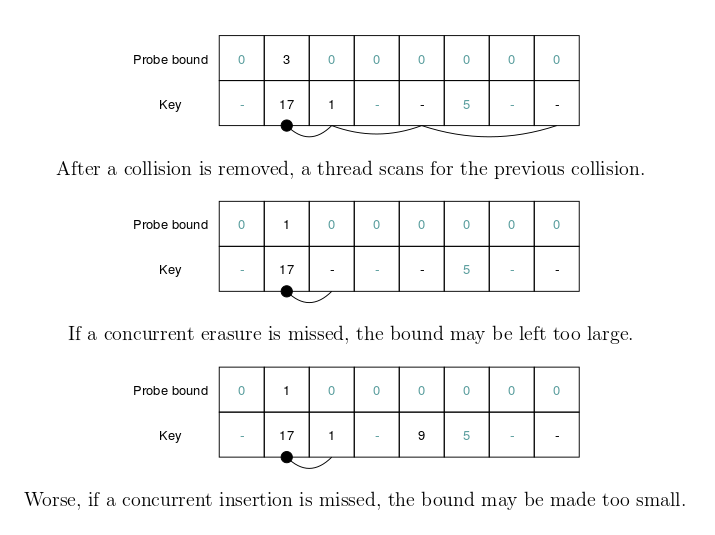
\includegraphics[scale=0.5]{non_blocking_1.png}
\caption{Problems maintaining a shared bound, after a collision is removed from the probe sequence}
\label{non_blocking_1}
\end{figure}

For this reason, we add a scanning bit for each probe bound, that we are able to update atomically, along with the probe bound. During insertion, threads just attempt to clear the bit and increase the bound if necessary. During deletions, a thread that is trying to erase a collision uses this bit to make sure that no other concurrent  updates have been made and that the probe bound has decreased correctly.

Every individual bucket holds the value and a state variable that helps resolve conflicts and synchronize concurrent operations, as described later. In order to prevent the ABA  problem, a version count is integrated along with each state variable.

In order to perform an insertion, a thread takes the following steps: First, it finds an empty bucket, stores the value and sets the state of that bucket to inserting. Then , it scans the probe sequence, looking for other threads inserting the same key, or a completed insertion of that key  ( characterized with the state member) . If a completed insertion is found, the thread sets its own working bucket to empty and the operation fails. If any other unfinished insertion operations are detected, the thread assists in the process of setting the first insertion found in the process to member and setting all the rest to collided. This operation is done concurrently by all threads working on the probe sequence, resulting in a lock –free algorithm where the delay of a single thread will not stall the others.

The main outline of the Insert and Assist operations are shown bellow.

\begin{lstlisting}

bool Insert(int key){
	h = Hash(k)
	i=-1
	do
		if ++i>= size 
			table is full
		<version, state> = Bucket(h,i)->vs
	while (! CAS (&Bucket(h,i)->vs,<version, empty>,<version, busy>))
	Bucket(h,i)->key=key
	while (!) {
		Bucket(h,i)->vs = <version, visible>
		ConditionallyRaiseBound(h,j)
		Bucket(h,i)->vs = <version, inserting>
		r = Assist(k,h,i,version)
		if Bucket(h,i).vs != <version, collided>
			return true
		if !r
			ConditionallyLowerBound(h,i)
			Bucket(h,i)->vs = <version+1, empty>
			return false
		version ++
	}
}

bool Assist(int k, int h, int i , int ver_i){
	max = GetProbeBound(h)
	for (j=0; j<max ;j++){
		if i!=j {
			<ver_j,state_j> = Bucket(h,j)->vs
			if state_j = inserting && Bucket(h,j)->key = k {
				if j<i{
					if Bucket(h,j)->vs = <ver_j,inserting){
					CAS(&Bucket(h,i)->vs, <ver_i,inserting>, <ver_i,collided>)
					return Assist(k,h,j,ver_j)
					}
				}else{
					if Bucket(h,i)->vs = <ver_i,inserting>
						CAS(&Bucket(h,j)->vs, <ver_j,inserting> ,<ver_j,collided>)
				}
			}
			<ver_j, state_j> = Bucket(h,j)->vs
			if state_j =  member && Bucket(h,j)->key = k{
				if Bucket(h,j)->vs = <ver_j, member>{
					CAS(&Bucket(h,i)->vs, <ver_i,inserting>,<ver_i, collided>)
					return false
				}
			}
		}
	CAS(&Bucket(h,i), <ver_i, inserting>, <ver_i, member>)
	return true
}

					
						
\end{lstlisting}

Figure \ref{non_blocking_2} is an example of how the algorithm detects and avoids collisions.

 %figure 9 apo paper
\begin{figure}
 \centering
  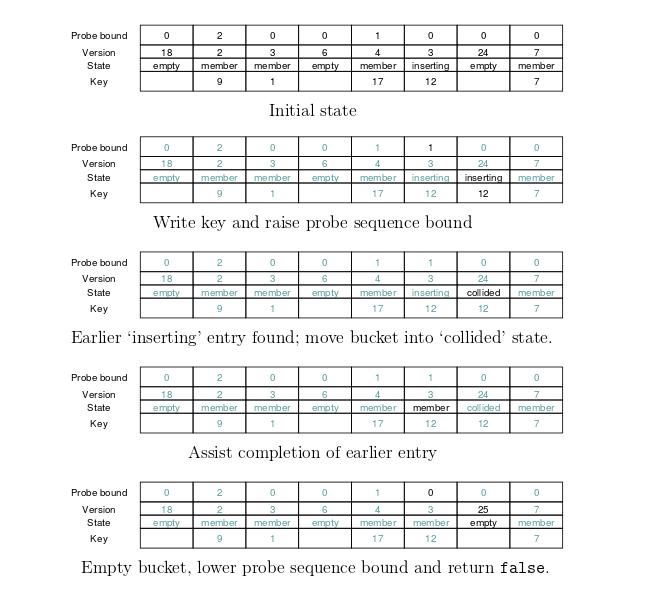
\includegraphics[scale=0.5]{non_blocking_2.png}
\caption{Inserting 12 using the lock-free algorithm.}
\label{non_blocking_2}
\end{figure}

The impact of the ABA problem is better understood from the following example of bad synchronization between inserting threads, in figure \ref{non_blocking_3} , that can be avoided with the use of version counters.

%figure 7 apo paper
\begin{figure}
 \centering
  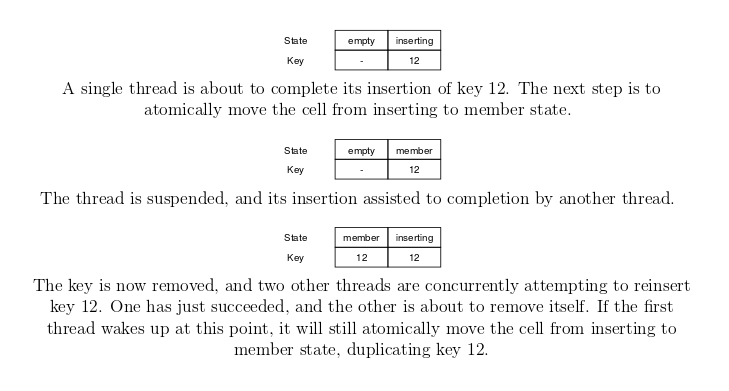
\includegraphics[scale=0.5]{non_blocking_3.png}
\caption{The effect of the ABA problem on concurrent assisting of operations.}
\label{non_blocking_3}
\end{figure}

This open addressing algorithm also requires bigger, partialy empty hash tables and resizing is again slow. However, if we know the aproximate size of the values inserted in advance, or if the workload consists mainly of lookups while instertions are rare, this implementation may perform better than the others,  mainly due to low it's small cache footprint that works very well with NUMA architectures. Figure \ref{hashes_non_blocking_perf} demonstrates that behaviour.

\begin{figure}
 \centering
  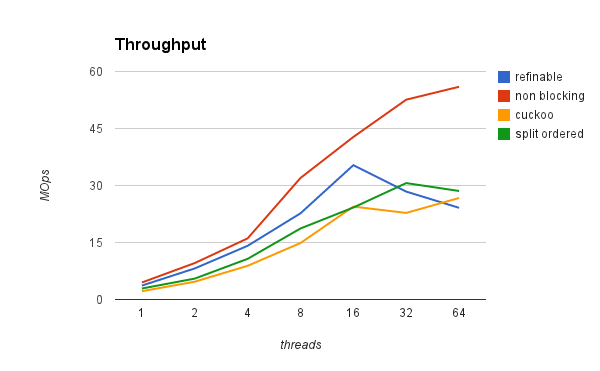
\includegraphics[scale=0.5]{hashes_non_blocking_perf.png}
\caption{Performance of the non blocking open addressing implementation}
\label{hashes_non_blocking_perf}
\end{figure}



\newpage
\small
\noindent
\selectlanguage{greek}  % mine
% mine -- maybe more text about copyrights, etc here.
\copyright \hspace{1em}(Εισάγετε έτος έκδοσης) Εθνικό Μετσόβιο Πολυτεχνείο.
\selectlanguage{english}  % mine
\textlatin{All rights reserved.}

\newpage
\selectlanguage{greek}  % mine
\printindex  % mine -- do you use one?
\nocite{*}
\bibliographystyle{babplain-fl}  %mine -- for name-surname order
\bibliography{references}  % mine -- the references.bib file
\end{document}
